% Should be <2 pages

% **Problems**

% **Needs to contain**
% - Hardware Description on a more detailed level

% **Structure**

% - Hardware section
%     - Overview
%     - Decisions
% - Software section
%     - Overview
%     - Decisions

The work in this paper is divided up into two major areas; the hardware and the software implementations. The aim of this section is to give an overview of the implementation and the design decisions made for each area.

\section{Hardware Implementation}

% Overview
A similar paper conducted at KTH earlier this year served as the main baseline for how the hardware was to be setup.\cite{hospital} The main components are the microcontroller, the scale as well as the ADC (Analog-to-Digital Converter). Apart from this, an adequate power source is needed to provide energy to all components. 

% Decisions

\subsection{Scale}
The scale used for this paper is a Tedea Huntleigh - Model 1022. It's a small and simple model, and the specific device used in this paper had a maximum capacity of \~50 kg.\cite{load-cell-data} In figure \ref{fig:wiring} we can see the labels of the four wires needed to hook up the load cell. The \textit{Input+} and \textit{Input-} signify the voltage input and ground. \cite{load-cell-spec} \textit{Output+} and \textit{Output-} will output a positive respectively a negative charge of \~1.5 voltage . During weighing, the internal resistance in the load cell will change ever so slightly, and the two outputs will have a small difference in the millivoltage range. This difference represents the weight measurement, and can be translated to a corresponding kg/lb value. In general, the more voltage the scale is supplied with, the greater this millivoltage range can be, which (in theory) means larger accuracy when weighing. Bear in mind that no two load cells are the same, and need to be calibrated to output the correct kg/lb value. Even though no calibrations were made to the load cell during this paper, an increase in the voltage provided to the load cell did correlate to an increased stability in the values produced. 

\begin{figure}[h]
	\centering
	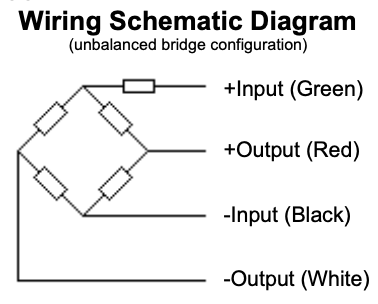
\includegraphics[width=0.3\textwidth]{load-cell-wiring.png}
	\caption{The wiring schematic for the load cell}
	\label{fig:wiring}
\end{figure}


\subsection{ADC}
To convert the millivoltage output from the load cell into a digital signal, an ADC is needed. The device used in this paper is an HX711, and apart from being a converter, it also serves as an amplifier for the load cell signal. We can see the front of the piece in figure \ref{fig:hx711}, and on the left side are the pinout where all the wires from the load cell should be connected. It's worth bearing in mind that the color coding of the wiring is not the same for all load cells, and the backside should be checked so that the connections made follow the correct wiring schematic. 

It outputs data via two of its pins, the DAT and the CLK. The CLK pin will output 0 if it's ready to send data, and 1 if it is not ready. When it is ready, the DAT pin will send  a series of 0s and 1s that can be converted from binary to a decimal value, which will then represent the output of the load scale.\cite{hx711-datasheet} Multiple code libraries have been written to handle this for the user, and the only thing left to implement is to specify which pins are being used by CLK and DAT respectively. For this paper, a library written for micropython was used.\cite{hx711-lopy}

\begin{figure}[h]
	\centering
	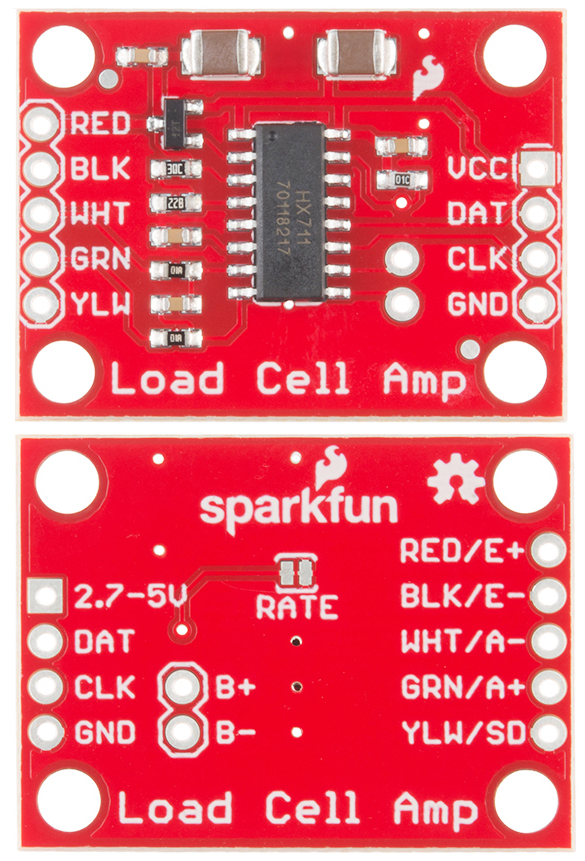
\includegraphics[width=0.3\textwidth]{hx711.png}
	\caption{The front and back of the HX711}
	\label{fig:hx711}
\end{figure}


\subsection{Microcontroller}
The microcontroller used for this paper was the FiPy development board from PyCom. It boasts a wide range of capabilities when it comes to communication protocols, NB-IoT being one of the five available.\cite{fipy-docs} With the supplied expansion board, connections via pinout is possible. It runs on micropython, which is an implementation of Python 3 optimized to run on microcontrollers.\cite{micropython}

\subsection{Power Source}
In the early stages of the project, the hardware was powered via USB cable from a computer. Since the USB was of type micro, the voltage output was at 5V. The benefit of this setup was a simple wiring schema where each component powered the next in line. The drawback was that the FiPy could only supply the ADC with 3V, which in turn affected the ADC's ability to read data from the load cell. During testing, the output rate of the raw data would be infrequent and erratic, sometimes taking several seconds to produce a single value. The values themselves did not correspond to increases and decreases in force being applied to the load cell, and would seemingly spike and crash at random. These problems were largely in part due to insufficient voltage being supplied to the ADC and load cell as later setups would reveal.

To remedy this, an approach using two different power sources was tried, where the ADC was powered by a wall outlet at a higher voltage, while the FiPy kept the USB. This resulted in electrical interference throughout the system, because of two different grounds being present in the circuit. The output rate of the data values had improved to a bit more stable rhythm than before, and the raw data values were a bit more responsive to the force applied to the load cell. 

\subsection{Wiring}
\begin{figure}[h]
	\centering
	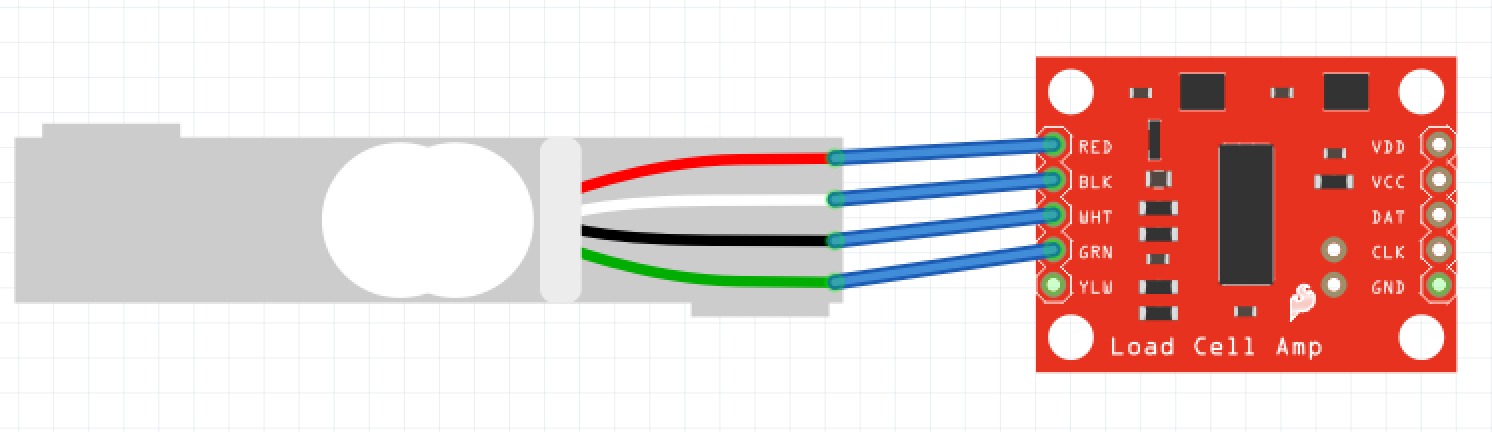
\includegraphics[width=0.6\textwidth]{load-cell_hx711.png}
	\caption{The load cell wired to the ADC}
	\label{fig:load-cell_hx711}
\end{figure}

\subsection{Failures}
During the first half of the project a faulty load cell was being used, which resulted in major delays of the hardware implementation. During the later half of the project no adequate solution to the problems with the power source could be devised in time for the practical testing of the hardware. Despite that no stable and satisfactory setup could be devised




\section{Software Implementation}



% To determine what we want to achieve in this aspect, it's useful to first define some behaviors from which we will base our assumptions on. In figure \ref{fig:linear} we see our base case, with a simple linear decline in data values. In figure \ref{fig:plat} we see data the goes through some changes periodically, but stabilizes itself between the changes. In figure \ref{fig:spikes} we see a clear linear decrease with some spikes in data values here and there, which we can assume to be faulty measurements.

% \subsection{Implementation}
% We're interested in modifying the data reading rate depending on the changes in data values. This can be done in a number of ways, but a simple start might be to measure the delta in the last \textit{x} amount of values and increase/decrease the rate depending on it's relation to delta. 

% To do this we need a \textit{short term buffer} of a fixed size that contains \textit{x} amount of recently read values in chronological order. This buffer should act as a FIFO-queue, so that the first element added to the buffer is the first one removed during an overflow. Measuring the delta of all the values in the buffer, we compare it to a threshold value that will either decrease, increase or maintain the current interval of reading data. When we say the delta of \textit{all} values in the buffer, we mean the delta between each data point summed up. Assuming a buffer of 10 values, we would calculate the sum as follows:

% $$\sum_{n=0}^{8} x_n - x_{n+1}$$

% Starting with figure \ref{fig:linear}, the values go from (100-0) in 100 data points on the x-axis. Calculating the delta for the first 10 values would be simple. The short term buffer would be: [100, 99, ..., 91]. The total delta would be (100-99) + (99 - 98) + ... + (92 - 91) = 10. For this example we can say that our determined threshold for decreasing our reading interval is $\geq 15$, and an increase at $\leq 5$. In our current example the reading rate is maintained. 

% In figure \ref{fig:plat} the slopes are steeper, and would thus generate a larger total delta. Assuming a buffer length of 10, the first 5 values would be 100, and the other 5 would be 75. Our delta calculation would give us a value of 25, which would warrant a increase in our reading rate. In figure \ref{fig:spikes} the calculation would work the same as as in \ref{fig:linear}, with the exception of some outlying data points. In regards to data reading rate, we can handle these values in two ways. Either we filter them in some way, or include them. Depending on the application, filtering can be easy. For example, perhaps we know that values $\geq$ 150 are impossible for our sensor, and thus we can manually check each values to see if they adhere to our specific bounds. Perhaps we know that such rapid changes in said values aren't possible, and we can filter them based on that. One way of doing this might be to calculate the average value of the short term buffer, and only allow new data within a range of  \textit{x} amount of units. Given the short term buffer [100, 99, ... 91], the average value would be 95.5. In our application we know that data points can only reasonably change with about ~20 units, assuming a minimum reading rate. We set the limit to 30 units to give the program some leeway. In either way, extreme data points can be filtered. 

% A valid question at this point is \textit{how often} we should perform this delta measurement, and of course the answer depends on the needs and workings of the application. Some applications might benefit from adjusting their reading rate very tightly, while others might only want to do this periodically. 

% To sum up the important design choices when considering how often the sensor should be polled, we considered:
% \begin{itemize}
% 	\item What values we \textbf{compare} our short-term delta to. When should we decrease, increase or maintain our current data reading rate.
% 	\item What values are \textbf{valid} in the context of our application.
% 	\item How \textbf{often} we should adjust our reading rate interval.
% \end{itemize}

% \section{Sensor Failure}

% \subsection{Behaviors}
% In the previous chapter we defined a sensor failure as a state where the sensors measures invalid data for such a period of time that the sensor isn't deemed functional. Functional can mean different things for different applications, such as that one successful reading an hour is enough for one case, while one successful read per second might not even be enough for another. The question of how to determine successful readings versus unsuccessful ones are beyond the scope of this paper and varies greatly from sensor to sensor. We will aim to implement one way of handling the device state when these faulty readings do occur.

% \begin{figure}[H]
% \centering
% 	\begin{subfigure}[b]{0.3\textwidth}
%     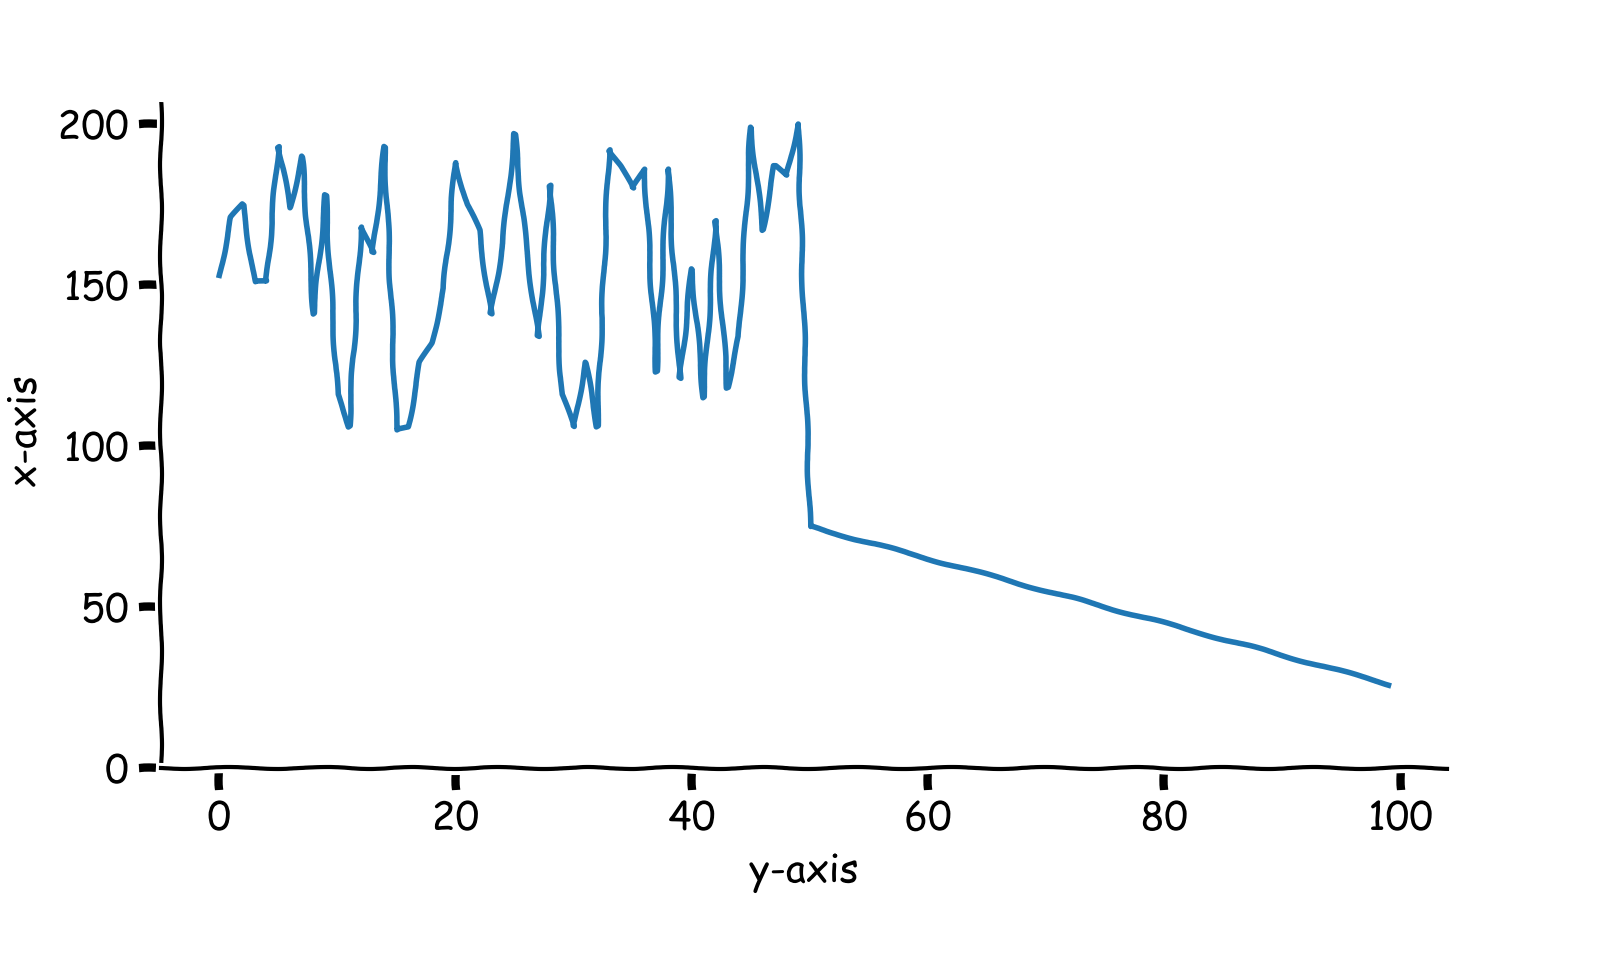
\includegraphics[width=\textwidth]{half_faulty_data.png}
%     \caption{Graph with some faulty data}
%     \label{fig:half_faulty}
% 	\end{subfigure}
% 	%
% 	\begin{subfigure}[b]{0.3\textwidth}
%     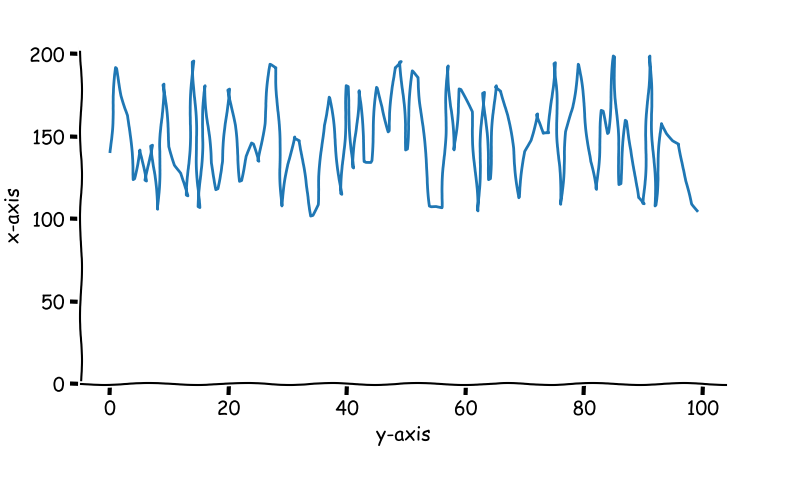
\includegraphics[width=\textwidth]{faulty_data.png}
%     \caption{Graph with only faulty data}
%     \label{fig:faulty}
% 	\end{subfigure}
% 	%
% 	\begin{subfigure}[b]{0.3\textwidth}
%     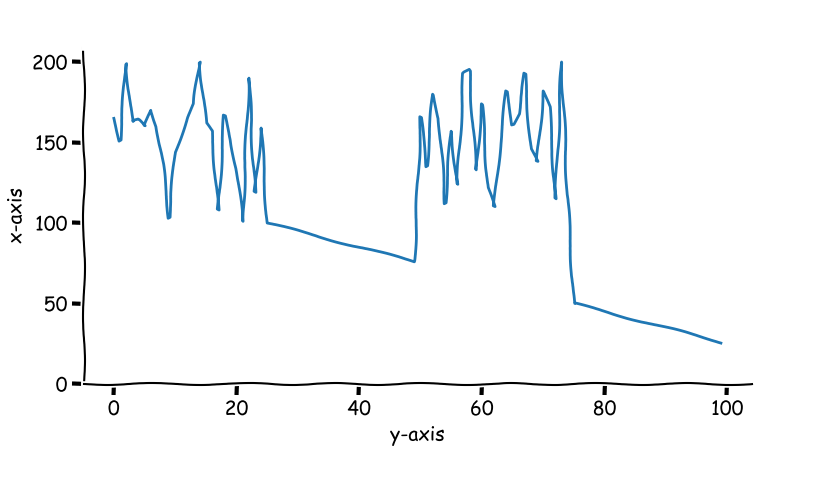
\includegraphics[width=\textwidth]{some_faulty.png}
%     \caption{Graph with two intervals of faulty data}
%     \label{fig:some_faulty}
% 	\end{subfigure}
% \end{figure}

% In fig \ref{fig:half_faulty}, the sensor first reads faulty data but then recovers  and starts producing valid data halfway through. In fig \ref{fig:faulty} all the data produced is faulty. In fig \ref{fig:some_faulty} there is one interval of faulty data followed by recovery, and then it repeats this pattern one more time.

% \subsection{Implementation}
% % TODO: Describe what to do at one failure
% Starting from figure \ref{fig:half_faulty} we receive faulty data from the sensor. Normally we might expect the occasional value to not be valid without raising any alarms, but after receiving 10 in a row 

% % TODO: Describe multiple failure levels & grace period


% \section{Sensor Disconnect}